\section{accel\_\-capture.c File Reference}
\label{accel__capture_8c}\index{accel_capture.c@{accel\_\-capture.c}}
{\tt \#include $<$avr/io.h$>$}\par
{\tt \#include $<$avr/interrupt.h$>$}\par
{\tt \#include \char`\"{}accel\_\-capture.h\char`\"{}}\par
{\tt \#include \char`\"{}globals.h\char`\"{}}\par


Include dependency graph for accel\_\-capture.c:\begin{figure}[H]
\begin{center}
\leavevmode
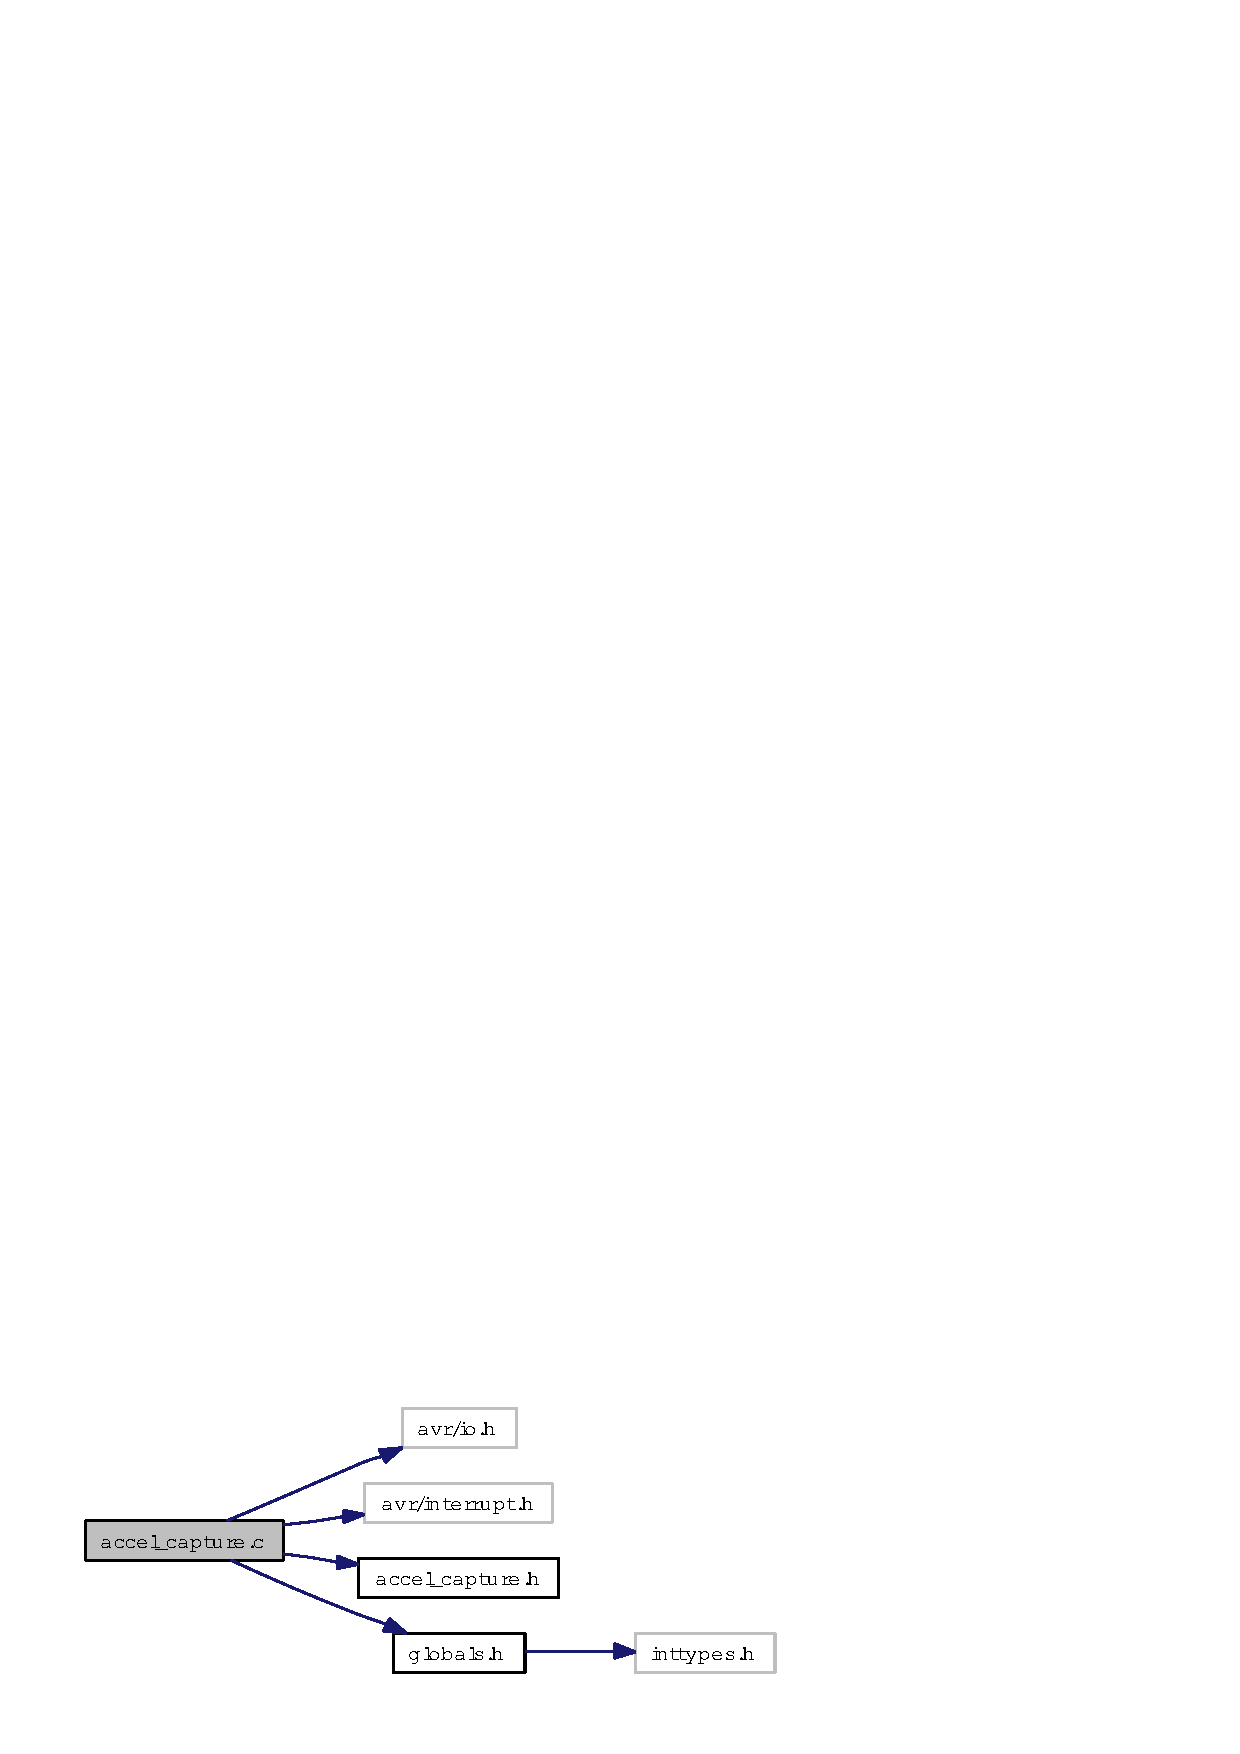
\includegraphics[width=188pt]{accel__capture_8c__incl}
\end{center}
\end{figure}
\subsection*{Functions}
\begin{CompactItemize}
\item 
{\bf SIGNAL} (SIG\_\-INPUT\_\-CAPTURE3)
\item 
void {\bf init\_\-accel\_\-capture} ()
\end{CompactItemize}


\subsection{Function Documentation}
\index{accel_capture.c@{accel\_\-capture.c}!SIGNAL@{SIGNAL}}
\index{SIGNAL@{SIGNAL}!accel_capture.c@{accel\_\-capture.c}}
\subsubsection{\setlength{\rightskip}{0pt plus 5cm}SIGNAL (SIG\_\-INPUT\_\-CAPTURE3)}\label{accel__capture_8c_3796dad092b974fdc241edd6f0849b83}




Definition at line 40 of file accel\_\-capture.c.

References accl\_\-high\_\-idx, accl\_\-high\_\-samples, accl\_\-low\_\-idx, accl\_\-low\_\-samples, and ACCL\_\-SAMPLES\_\-BUFSIZE.